\documentclass[10pt,twocolumn]{article}
\usepackage[utf8]{inputenc}
\usepackage{tabu}
\usepackage{caption}
\usepackage{booktabs}
\usepackage[margin=20mm]{geometry}
\usepackage{amsmath}
\usepackage{graphicx}
\usepackage{caption}
\usepackage{textcomp}
\usepackage{subcaption}
\usepackage{amssymb}
\usepackage{multicol}
\usepackage{authblk}
\usepackage{sectsty}
\usepackage{url}
\usepackage[
    backend=biber,
    style=authoryear,
    citestyle=authoryear-comp,
    natbib ]{biblatex}
\geometry{letterpaper}
\geometry{portrait}

\addbibresource{reference.bib}

% \sectionfont{\fontsize{12}{10}\selectfont}
% \subsectionfont{\fontsize{10}{10}\selectfont}

\title{Bayesian decoding and confidence estimation for deep combinatorial sequence indexing with Pheniqs}
\author[1]{Lior Galanti}
\author[3]{Dennis Shasha}
\author[2]{Nizar Drou}
\author[1,2]{Kristin C. Gunsalus\thanks{Contact: lg1883@nyu.edu, kcg1@nyu.edu}}
\affil[1]{\footnotesize{Center for Genomics \& System Biology, Department of Biology, New York University, New York, 10003, United States}}
\affil[2]{\footnotesize{NYU Abu Dhabi Center for Genomics \& System Biology, Division of Biological Sciences, Abu Dhabi, United Arab Emirates}}
\affil[3]{\footnotesize{Courant Institute, Department of Computer Science, New York University, New York, 10003, United States}}

\begin{document}

\maketitle

\section*{Abstract}
%
\textbf{Background:} Systems biology increasingly relies on deep sequencing with combinatorial index tags called barcodes to associate individual biological sequences with their respective sample, individual cell, and/or molecule. Accurate data interpretation critically depends on discerning the correct origin of each sequence of interest, and hence on the final classification confidence. This, in turn, is cumulatively impacted by the decoding confidence of the various barcodes. Preserving a classification quality score is especially desirable when the decision to assign or discard a read depends on factors only available downstream. These may include the observed distribution of expected barcodes within a mixture of bulk sequencing samples, or the number of individual cells that can be reliably detected in single-cell sequencing experiments. Despite these advantages, computation and reporting of decoding confidence scores have not been widely adopted. To improve overall performance at this critical stage of sequence analysis, we have developed a flexible and robustly engineered software package, Pheniqs, that supports arbitrarily complex barcoding schemes and enables standardized reporting of decoded index sequences with classification confidence scores.\\
%
\textbf{Results:} Pheniqs implements both a standard minimum distance decoder and a probabilistic decoder that classifies sequence reads based on the full posterior probability of observed barcode indexes. Pheniqs consults basecalling quality scores and prior distributions to compute the posterior decoding error probability of individual barcodes and reports the resulting barcode sequences and confidence scores in SAM auxiliary tags. Performance evaluation using synthetic data indicates that Pheniqs achieves greater accuracy than minimum distance or simple maximum likelihood estimation decoding by correctly computing the full posterior classification probability.\\
%
\textbf{Conclusions:}
Decoding barcodes using full posterior probabilities is more accurate than available methods. Individual decoding confidence scores can be combined into a combinatorial decoding confidence. An optimized multithreaded implementation assures that Pheniqs is also faster and scales better with large and complex barcode sets than existing tools. Pheniqs can be extended with new error models and relies on intuitive confidence thresholds for fine-tuning decoding accuracy.\\

\section*{Background}
% The Background section should explain the relevant context and the specific issue that the software described is intended to address.
High-throughput sequencing with multiplexed sample barcodes is now standard practice, and single-cell applications are rapidly gaining in popularity. To enhance resolution and to control for different quantification biases, supplemental barcodes have been introduced to tag the individual cell and molecule from which sequence reads originate. Increasingly complex barcoding schemes are being devised to accommodate new experimental applications \citep{doi:10.1038/s41576-019-0093-7}, and cellular indexing protocols may include several successive rounds of barcoding, increasing the potential combinatorial space exponentially \citep{doi:10.1126/science.aam8940}. Uneven barcode distributions and noise reads that do not belong to any of the classes are common, and add to the challenge of sequence classification.

Existing barcode decoding tools were designed to handle reads that are multiplexed with a single, relatively small, set of sample indexes and thus are not well adapted to the rising use of novel experimental designs with custom multi-component barcoding schemes and associated complexities of the sequence data. Pheniqs overcomes many of the limitations of these first-generation decoders by rethinking key aspects of current decoding requirements: scalability, assumptions about the number of tags and their location, and the ability to explicitly account for base calling quality scores, prevalent foreign or noise sequences, and uneven barcode distributions.

Pheniqs (\textbf{PH}ilology \textbf{EN}coder w\textbf{I}th \textbf{Q}uality \textbf{S}tatistics, pronounced \textit{phoenix}) combines a generic and extensible approach to barcode decoding with flexible configuration options that easily accommodate custom applications. A robust and efficient code base and extensive documentation support individual installations and large-scale production facilities alike. Pheniqs implements both a standard minimum distance decoder (MDD) and a probabilistic decoder that consults base-calling quality scores as well as priors to compute the full posterior decoding probability for classification rather than a simple maximum likelihood estimate.

Several existing tools for demultiplexing barcode sets are currently available. Illumina's bcl2fastq tool only accepts input in the proprietary Illumina BCL format. It is specifically geared toward sample demultiplexing of Illumina data and relies on quality assessment procedures that are not obviously accessible to end-users. Standalone, peer reviewed, classifiers include deML \citep{doi:10.1093/bioinformatics/btu719}, Bayexer \citep{doi:10.1093/bioinformatics/btv501}, and Axe \citep{doi:10.1093/bioinformatics/bty432}. DeML is capable of handling a single barcode set with either one or two segments. While it consults base calling qualities and reports classification scores in Sequence Alignment/Map (SAM) \citep{doi:10.1093/bioinformatics/btp352} auxiliary tags, it does not accurately reflect the probability of correct classification. Instead, it estimates maximum likelihood only for the top candidates that are within a short Hamming distance, under restrictive assumptions that do not hold in most complex cellular indexing designs -- specifically, that barcodes are uniformly distributed, and that foreign sequences (i.e. those that should not match any barcode) are extremely rare. Bayexer attempts to train a naive Bayes classifier by studying the error pattern when the insert sequence is shorter than the read length and results in a second observation of the barcode. Although this approach can potentially increase accuracy in those specific cases, it is not applicable to general barcode decoding and the tool fails to produce output when such redundancy is not present. Axe uses a set of pre-computed prefix trees to find a match within a given Hamming distance and can partially handle barcodes that differ in length. Although this method can be very fast, it ignores quality scores, and it is highly sensitive to upstream errors in the prefix and so sacrifices accuracy. None of the above tools account for the prior sample distribution or foreign sequence frequency, compute or report the posterior classification probability for individual reads, or handle multiple indexes from both sample and cellular tags. In addition, they all lack the ability to address read fragments in arbitrary offsets or to decode barcodes with more than two segments, and so often require custom preprocessing to reposition the barcode.

\section*{Implementation}
% This should include a description of the overall architecture of the software implementation, along with details of any critical issues and how they were addressed.

Pheniqs is distributed as a compiled binary with a command line interface that accepts a JSON encoded configuration file. Using a familiar syntax that mimics python array slicing Pheniqs can decode multiple barcodes located anywhere in the sequencing read. It uses tokens extracted from read segments by addressing either the 5’ end, 3’ end or both and optionally reverse complemented to construct the output template segments, as well as sample, cellular and molecular barcodes (Figure~\ref{fig:16}). This generic approach allows for arbitrary manipulation that accommodates any potential barcoding scheme and experimental design and often obviates the need for pre and post processing.

By directly interfacing with the low level HTSlib C API Pheniqs can read, write, and manipulate either uncompressed or gzip compressed FASTQ files as well as the SAM file format or any of its binary compressed variants BAM and CRAM. Unlike FASTQ, the SAM format can encode sequencing data in a single, smaller file that supports richer metadata annotations. To maximize multithreading capacity Pheniqs implements mutual exclusive locking on double IO buffers. Rotating the two buffers allows threads computing the posterior probabilities to work without waiting for threads writing output. When integrated into a pipeline, Pheniqs can take advantage of POSIX standard streams to avoid the speed and storage bottlenecks associated with reading and writing temporary files.

Pheniqs reports the decoded sample, cellular and molecular barcodes as well as their corresponding quality scores and the posterior decoding error probability in SAM auxiliary tags. It supports declaring standard SAM read groups to be associated with the sample barcodes and can optionally perform an exhaustive quality assessment during processing that is included in the final report.

\subsection*{Probabilistic decoding}

Classification based on barcodes involves extracting a subsequence $r$ from an observed read, along with the basecall quality scores associated with the individual nucleobases in $r$, and decoding the original sequence $s$. Let $r \in \{A,C,G,T,N\}^n$ be an observed sequence of length $n$ extracted from the read and $\mathcal{B} \subseteq \{A,C,G,T\}^n$ a given set of distinct barcodes where each $b \in \mathcal{B}$ identifies an individual class. A decoder is denoted as a decision function $\phi: \{A,C,G,T,N\}^n \mapsto \mathcal{B} \cup \varepsilon$ where $\varepsilon$ denotes a decoding failure for a foreign sequence, i.e., $s \notin \mathcal{B}$.

A maximum likelihood decoder will identify the barcode $\hat{b} \in \mathcal{B}$ which maximizes the posterior probability that $\hat{b}$ was sequenced given that $r$ was observed, assuming it is not a foreign sequence.
%
\begin{equation}
\hat{b} = \operatorname*{arg\,max}_{b \in \mathcal{B}} P(b|r)
\end{equation}
%
Applying Bayes' rule we can compute $P(b|r)$ using
%
\begin{equation}
P(b|r) = \frac{P(r|b)P(b)}{P(r|b \notin \mathcal{B})P_{\varepsilon} + \sum_{b' \in \mathcal{B}} P(r|b')P(b')}
\end{equation}
%
where $P_\varepsilon$ is the prior probability of encountering foreign sequences and $P(r|b \notin \mathcal{B}) = 1/4^n$, as foreign sequences are assumed to produce random observations.

The \emph{Phred-adjusted maximum likelihood decoder (PAMLD)} implemented by Pheniqs solves \textbf{Equation 2} by computing $P(r|b)$ for each $b \in \mathcal{B}$ from the base calling quality scores \citep{doi:10.1093/bioinformatics/btv401}. $P(b)$, the expected fraction of reads identified by $b$, can be either estimated from the data or provided \emph{a priori} by the user.

When $P(r|\hat{b}) < 1/4^n$ the initial evidence supporting the classification is inferior to that provided by a random sequence, indicating the $\hat{b}$ recovered in \textbf{Equation 1} is more likely to be noise. The \emph{noise filter} considers those a decoding failure without further consideration.
%
In addition, the \emph{confidence filter} declares a failure if $P(\hat{b}|r) \leq C$ where $C$ is a user provided confidence threshold for the minimum acceptable probability of a correct decoding (Figure~\ref{fig:03}). The probability of a decoding error is
%
\begin{equation}
P_{\text{decoding\_error}}(\hat{b}, r) = 1 - P(\hat{b}|r)
\end{equation}
%
Therefore, directly estimating $P(\hat{b}|r)$ allows Pheniqs to report an intuitive classification confidence for every read, while the governing threshold $C$ allows researchers to choose between assignment confidence and yield of classified reads.

By contrast, deML \citep{doi:10.1093/bioinformatics/btu719} assumes that $P_{\varepsilon}$ is infinitesimally small and that samples are uniformly pooled, thereby suggesting that for every $b \in \mathcal{B}$
%
\begin{equation}
P(b) = \frac{1 - P_{\varepsilon}}{|\mathcal{B}|} %\mathrel{\mathop{=}\limits_{P_{\varepsilon} \to 0}}
\approx \frac{1}{|\mathcal{B}|}
\end{equation}
%
Under such conditions $P(b|r) \propto P(r|b)$ and \textbf{Equation 1} can be simplified to
%
\begin{equation}
\hat{b} = \operatorname*{arg\,max}_{b \in \mathcal{B}} P(r|b)
\end{equation}
%
While such assumptions simplify maximum likelihood estimation of $\hat{b}$, they are often grossly imprecise. A relatively low yield in (e.g. single-cell) experiments that rely on several layers of combinatorial indexing often results in an extremely uneven barcode distribution, with $P_{\varepsilon}$ representing a significant portion of the sequenced DNA. Furthermore, implementations that refrain from computing $P(\hat{b}|r)$ can not report the posterior classification probability.

\subsection*{Prior estimation}

A \emph{high confidence estimator} uses statistics from a prelimenatry PAMLD decoding run to estimate the noise prior $P_{\varepsilon}$ and the individual barcode priors $P(b)$ for each $b \in \mathcal{B}$. It assumes that \emph{low confidence} reads, i.e. reads that passed the \emph{noise filter} but failed the \emph{confidence filter}, and \emph{high confidence} reads, i.e. reads that passed both filters, come from the same distribution. The priors are estimated only from the \emph{high confidence} reads.

Let $S_{\varepsilon}$ be the number of reads filtered by the \emph{noise filter}, $S_{b}$ the number of reads classified to $b$ with confidence higher than $C$ and $S_\mathcal{B} = \sum_{b \in \mathcal{B}} S_{b}$. An estimator for the noise prior is

%
\begin{equation}
\hat{P_{\varepsilon}} = \frac{S_{\varepsilon}}{S_{\varepsilon} + S_\mathcal{B}}
\end{equation}
%

and for an individual barcode is

%
\begin{equation}
\hat{P(b)} = \frac{S_{b}}{S_{\varepsilon} + S_\mathcal{B}}
\end{equation}
%

\section*{Results}
% This should include the findings of the study including, if appropriate, results of statistical analysis which must be included either in the text or as tables and figures. This section may be combined with the Discussion section for Software articles.
% The user interface should be described and a discussion of the intended uses of the software, and the benefits that are envisioned, should be included, together with data on how its performance and functionality compare with, and improve, on functionally similar existing software. A case study of the use of the software may be presented. The planned future development of new features, if any, should be mentioned.

\subsection*{Accuracy analysis on synthetic data}


We used the run published with deML to simulate barcoded sequence reads. Since indel errors occur at a much lower rate than substitutions \citep{doi:10.1038/s41598-018-29325-6} we only simulated substitution errors. On a \emph{first} step we simulated barcoded sequence reads by replacing the barcode nucleotides on each read with a perfect barcode sequence sampled from a prior distribution. To simulate foreign sequences we replaced a barcode with a sequence from a random offset on the \emph{PhiX174} genome. On a \emph{second} step we simulated substitution errors by introducing an error on a nucleobase according to the base call quality score and substitution frequencies made available with LRSim\citep{doi:10.1016/j.csbj.2017.10.002}. To simulate variable overall error rate we recalibrated the quality scores on a file produced in the \emph{first} step before simulating substitution errors in the \emph{second} step. See Figure~\ref{fig:14} for quality score distributions.

Each barcode and the undetermined class was evaluated as a binary classifier, so a correct assignment was counted as a true positive ($TP$) while an incorrect assignment was counted as a false negative ($FN$) for the correct class and as a false positive ($FP$) for the incorrectly assigned class. We then summed up the values from all classes and computed the \emph{precision} ($\frac{TP}{FP + TP}$), \emph{recall} ($\frac{TP}{FN + TP}$) and \emph{F-score} (harmonic average of the precision and recall). Reads that were marked as failing quality control were considered to be unclassified for this analysis. For each simulated file we classified the reads with the following consifurations: Pheniqs with MDD default settings(MDD), Pheniqs with PAMLD default settings(PAMLD uniform), Pheniqs with the true priors(PAMLD true), Pheniqs with \emph{high confidence estimated} priors(PAMLD estimated), and deML with default settings(deML). To computed the \emph{high confidence estimated} we used a priliminary run with the default configuration, i.e. a uniform barcode distribution and 0.05 noise.

Figure~\ref{fig:01} shows the F-score mesured for different overall error rates on the barcode cycles. MDD is clearly inferior to the probabilistic decders. Figure~\ref{fig:02} shows results only for the probabilistic decders. PAMLD is more accurate than both MDD and deML, in either configurations. As expected, the true prior performs the best but the \emph{high confidence} estimated prior is almost as good.

Figure~\ref{fig:12} shows the accumulated error in \emph{high confidence} prior estimation with barcodes binned by the true frequency. See figure~\ref{fig:13} for the true barcode frequency distribution and binning. The error in estimation is bellow 0.1\% for rates lower than 1 per 1000, the expected error rate on most Illumina platforms.  $\hat{P_{\varepsilon}}$ is consistantly over estimated by this method, which is the main drive of the under estimation of the individual barcodes. As the overall error rate increases, basecall quality on the barcode cycles can be poor enough that any substitution will cause the read to fail the \emph{noise filter}. This suggests that platforms with high error rates would benefit from prior estimation that accounts for this. This suggests the decoder using the estimated prior should underperform the true prior when error rates are high.

An often interesting presepective for a reasearcher is looking at results for \emph{classified} reads only - true barcoded or noise reads that were classified to a barcode. Figure~\ref{fig:05} shows FDR, MR and F-score for \emph{classified} reads only. Filtering noise helps Pheniqs outperform deML in any configuration. Figure~\ref{fig:06} shows the lower end of the FDR plot from Figure~\ref{fig:05} and includes MDD. In the range relevent to most Illumina runs, PAMLD has lower FDR than even MDD. In Figure~\ref{fig:07} results for \emph{classified} reads binned into 4 classes by their relative prior show the effect of the priors. Knowledge about the priors significantly reduce FDR but also marginally increase MR for reads in very rare classes (lower than 0.001). This is because a prior lower than the uniform penalises a class so reads are less likely to be classified to it. Reads with a prior similar to the uniform (0.001 to 0.03) show the same improvement in FDR but PAMLD already has better MR than deML. The default configuration favours this class so it has lower MR at the cost of higher FDR. Reads from slighty overrepresented classes show improved FDR when compared to default but slightly elevated MR when comapred to deML. The last bin includes only the control, which is the most overrepresented at 32\% of the run. where the priored PAMLD show the oposite trend of elevated FDR with improved MR. Figure~\ref{fig:08} shows that the behaviou is similar on the lower end relevent to most Illumina runs.

To evaluate noise filtering we look at \emph{classifiable} reads only - true barcoded reads, correctly classfied or not, and \emph{unclassfied} reads - reads classified as noise or failing quality control. Figure~\ref{fig:03} shows FDR, MR and F-score for \emph{classifiable} reads only, removing all true noise reads from the analysis. The default PAMLD is missclassifying more true reads than deML, although the priored configuration is still the most accurate. We can see this is partially due to the noise filter in figure~\ref{fig:09} that shows FDR, MR and F-score for \emph{unclassfied} reads only. PAMLD decoders classify more true barcoded reads as noise than deML when overall error is low. This is a side effect of noise filtering: If evidence supporting the class with the highest posterior is inferior to that provided by a random sequence the noise filter will reject the read even if the posterior is high. It is arguable that such reads have very weak evidence for classification. Zooming on the error rate range relevent for the Illumina platform, Figure~\ref{fig:10} shows that PAMLD filters noise better than even MDD, while Figure~\ref{fig:11} shows that priored PAMLD handles noise better than both the default and deML in both FDR and MR.

\subsection*{Runtime Speed and Memory evaluation}

To evaluate speed and memory usage we used a single lane from an Illumina NovaSeq, one the highest throughput instruments available today. 151 cycles were sequenced on each of the two template segments and 8 cycles on each of the i7 and i5 index segments. The lane conatined 94 multiplexed libraries with barcodes on the standard i7 and i5 segments. Bechmarks were executed on an Intel(R) Xeon(R) CPU E5-2690 v4 @ 2.60GHz with 14 cores and 28 threads.

Basecalling the lane with bcl2fastq yielded 11,578,868,372 dual indexed paired that passed quality filtering and took 47 minutes. bcl2fastq produces reads with segments split over four gzip compressed FASTQ files that were used as input. The choice of output has impact on performance so Pheniqs was benchmarked producing a variety of output layouts in several file formats. Figure~\ref{fig:15} shows speed and memory results. Pheniqs performs fastest when producing interleaved BAM output in 3:10 hours. Spliting output to multiple FASTQ files was slightly slower with CRAM being the slowest taking a little over 4 hours. CRAM uses several compression algorithms that are more agressive than gzip and produces smaller files, so the slight slowdown is expected. deML could only produce FASTQ output with FASTQ input so we could not test bam output. Lacking support for multithreading deML took almost 80 hours to decode the lane, at least 20 times longer than pheniqs. The pheniqs speed improvement is almost linear in the number of cores, even though it computes the full posterior probability. Pheniqs uses very little memory when writing to a single file, depending on the size of the IO buffers. When writing to multiple files each file is allocated a sperate IO buffer and memory consumption increases lineraly.

\section*{Conclusion}
% This should state clearly the main conclusions and provide an explanation of the importance and relevance of the case, data, opinion, database or software reported.
Decoding barcodes using full posterior probabilities is more accurate than available methods. Pheniqs offers an implementation faster and more scalable than existing tools. Pheniqs can be extended with new error models and relies on intuitive confidence thresholds for fine-tuning decoding accuracy. Individual decoding confidence scores can be combined into a combinatorial decoding confidence.

\section*{Availability and requirements}

\begin{itemize}
  \item \textbf{Project name:} Pheniqs
  \item \textbf{Project home page:} \url{http://biosails.github.io/pheniqs}
  \item \textbf{Operating systems:} Linux, MacOS.
  \item \textbf{Programming language:} C++11, Python 3.
  \item \textbf{Other requirements:} clang, gcc 4.8 or newer.
  \item \textbf{License:} AGPL-3.0.
  \item \textbf{Restrictions to use by non-academics:} licence needed
\end{itemize}

\section*{Acknowledgments}

We are grateful to Kapil Thadani and Or Biran for discussions on the statistical evaluation and mathematical notation; Alan Twaddle for his feedback on the user manual and his help with benchmark analysis and figure preparation; to Jillian Rowe for her assistance with Conda packaging, the dockerized distribution, and continuous integration and to Giuseppe Saldi for his insightful comments.

\section*{Funding}

This work was supported by a grant from the New York University Abu Dhabi (NYUAD) Research Institute to the NYUAD Center for Genomics and Systems Biology and by other research funding from NYUAD to KCG.

\section*{References}
\printbibliography[heading=none]

\section*{Figures}

\begin{figure}[htbp]
\centering
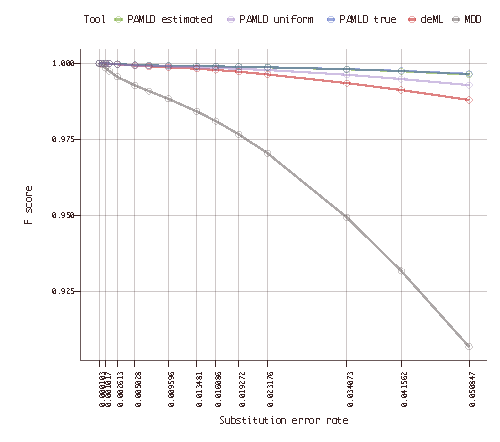
\includegraphics[keepaspectratio,scale=1]{../plot/1_overall_0550_mdd}
\caption{ \footnotesize{ \textbf{Decoding F-score.} Minium distance decoding is clearly inferior to the probabilistic decders. } }
\label{fig:01}
\end{figure}

\begin{figure}[htbp]
\centering
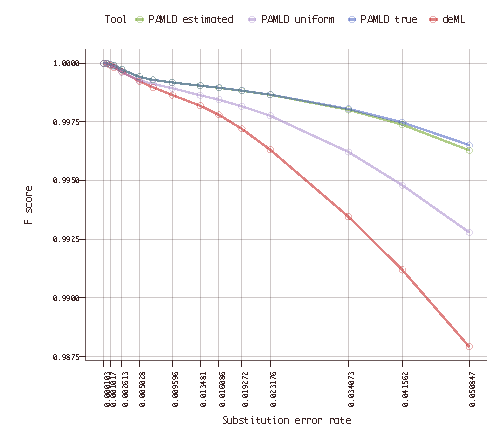
\includegraphics[keepaspectratio,scale=1]{../plot/2_overall_0550}
\caption{\footnotesize{\textbf{Probabilistic decoding F-score.} PAMLD is more accurate than both MDD and deML. The true prior performs the best but the \emph{high confidence} estimated prior is almost as good. } }
\label{fig:02}
\end{figure}

\begin{figure*}[htbp]
\centering
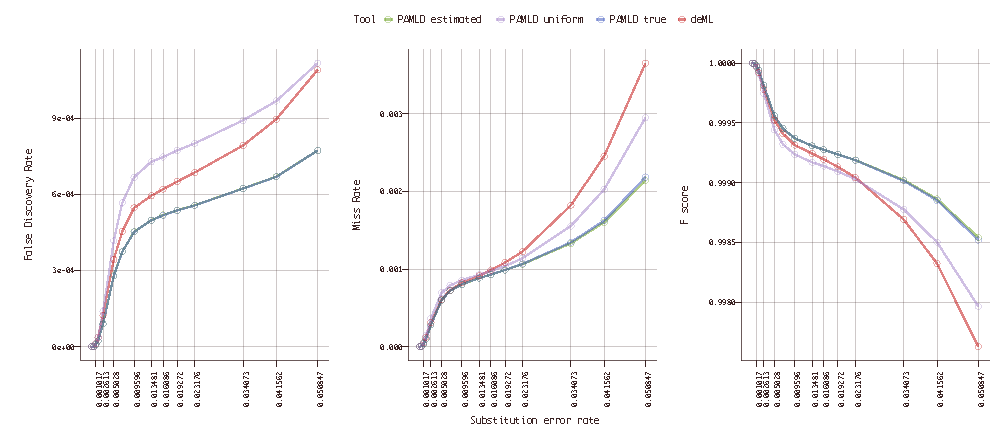
\includegraphics[keepaspectratio,scale=1]{../plot/3_classifiable_accuracy_0550}
\caption{\footnotesize{\textbf{Accuracy for classifiable reads only.} \emph{classifiable} reads are all true barcoded reads, correctly classfied or not.
} }
\label{fig:03}
\end{figure*}

% \begin{figure*}[htbp]
% \centering
% 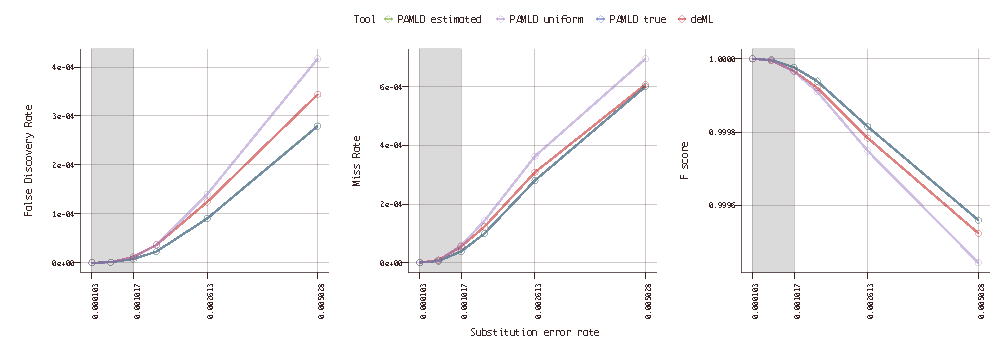
\includegraphics[keepaspectratio,scale=1]{../plot/4_classifiable_accuracy_0060}
% \caption{\footnotesize{\textbf{Accuracy for classifiable reads only closeup.} } }
% \label{fig:04}
% \end{figure*}

\begin{figure*}[htbp]
\centering
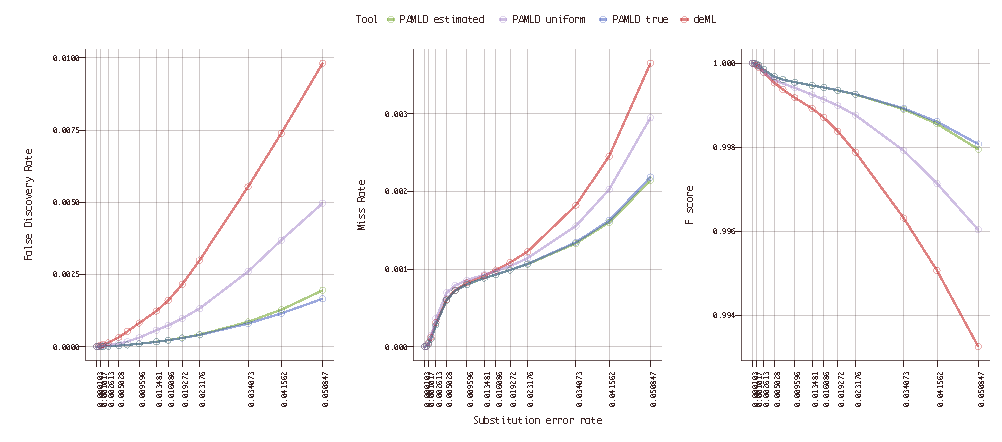
\includegraphics[keepaspectratio,scale=1]{../plot/5_classified_accuracy_0550}
\caption{\footnotesize{\textbf{Accuracy for classified reads only.} \emph{classified} reads are all true barcoded and noise reads that were classified to a barcode. } }
\label{fig:05}
\end{figure*}

\begin{figure*}[htbp]
\centering
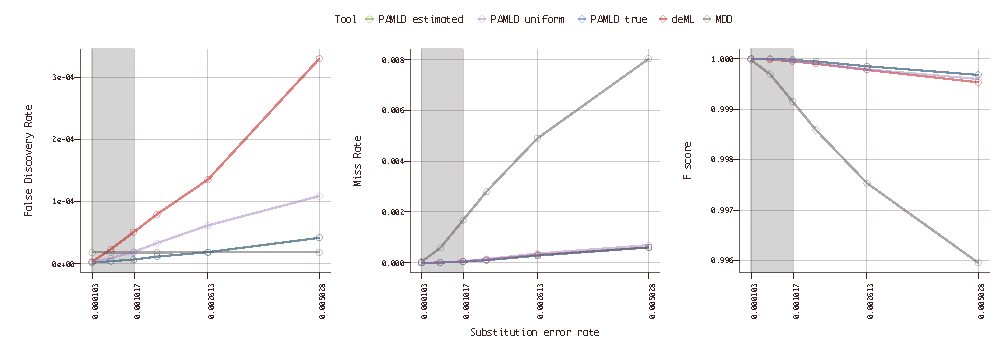
\includegraphics[keepaspectratio,scale=1]{../plot/6_classified_accuracy_0060_mdd}
\caption{\footnotesize{\textbf{Accuracy for classified reads only closeup with mdd.} } }
\label{fig:06}
\end{figure*}

\begin{figure*}[htbp]
\centering
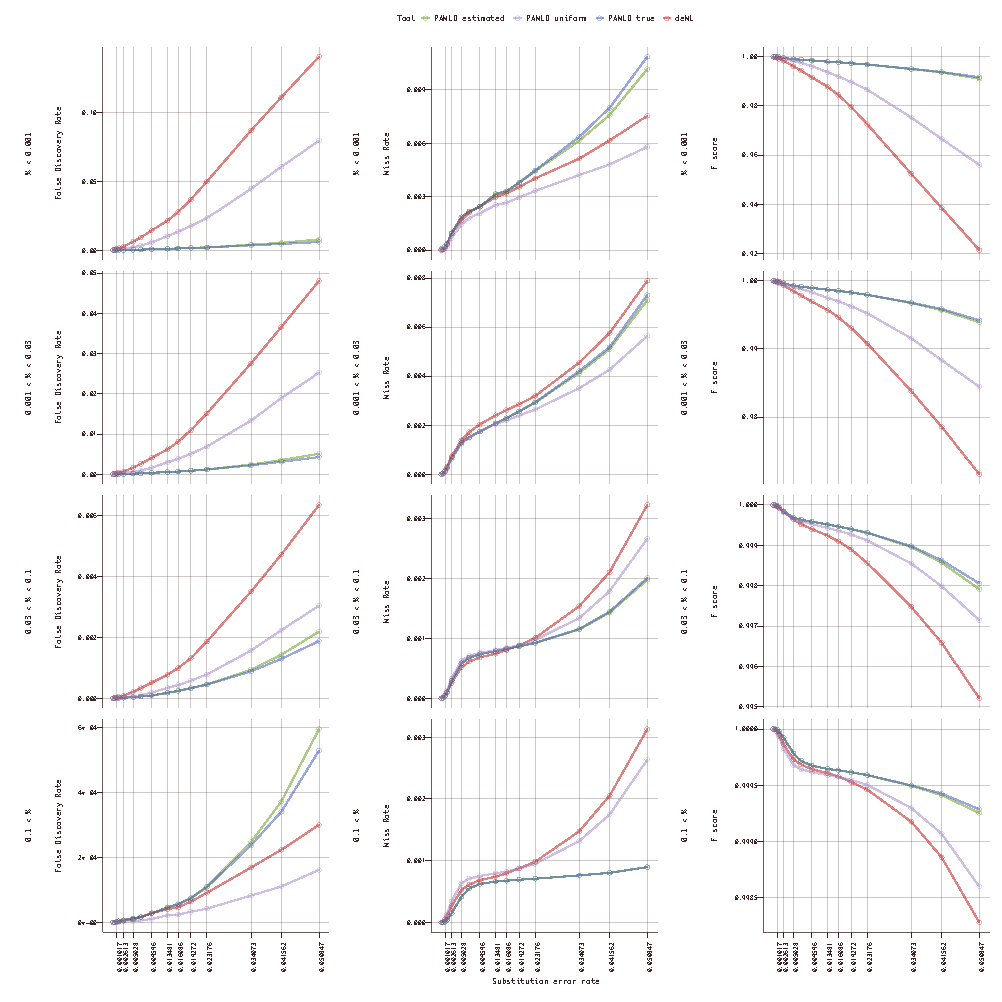
\includegraphics[keepaspectratio,scale=1]{../plot/7_classified_accuracy_0550_binned}
\caption{\footnotesize{\textbf{Accuracy for binned classified reads.} } }
\label{fig:07}
\end{figure*}

\begin{figure*}[htbp]
\centering
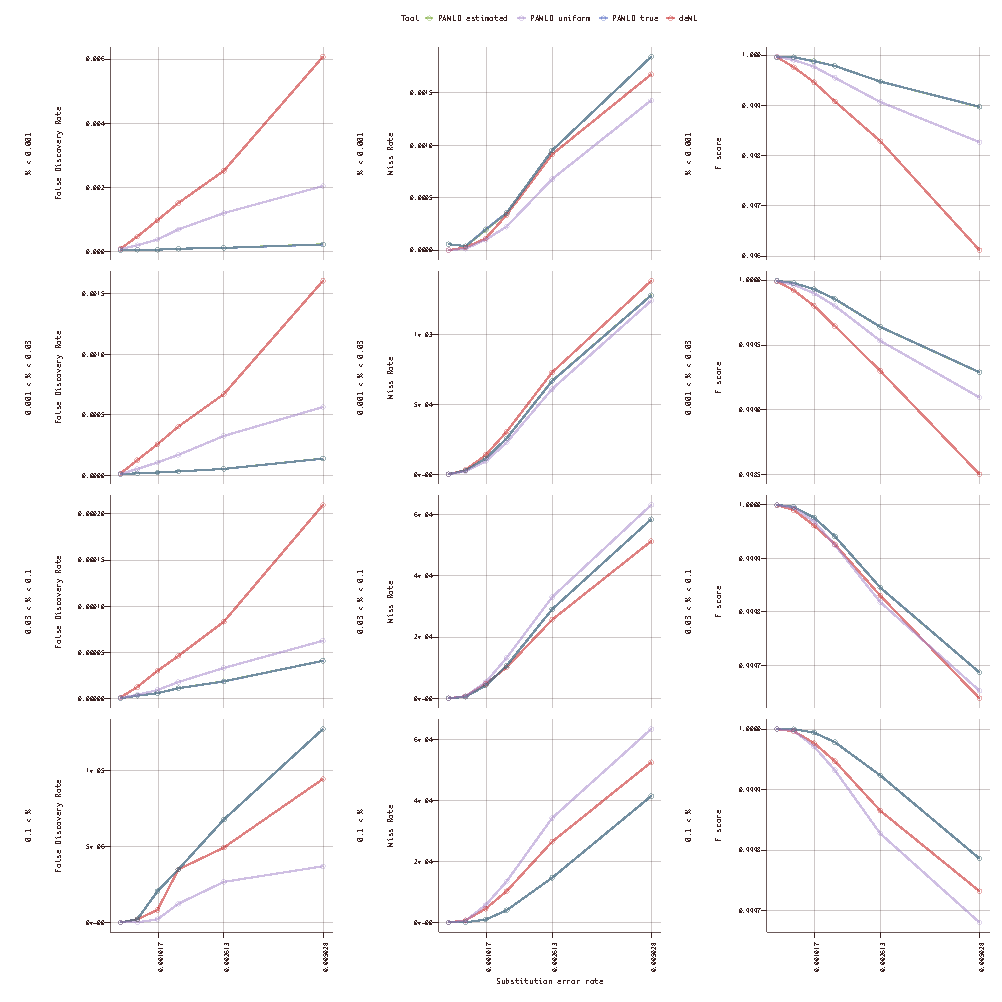
\includegraphics[keepaspectratio,scale=1]{../plot/8_classified_accuracy_0060_binned}
\caption{\footnotesize{\textbf{Accuracy for binned classified reads closeup.} } }
\label{fig:08}
\end{figure*}

\begin{figure*}[htbp]
\centering
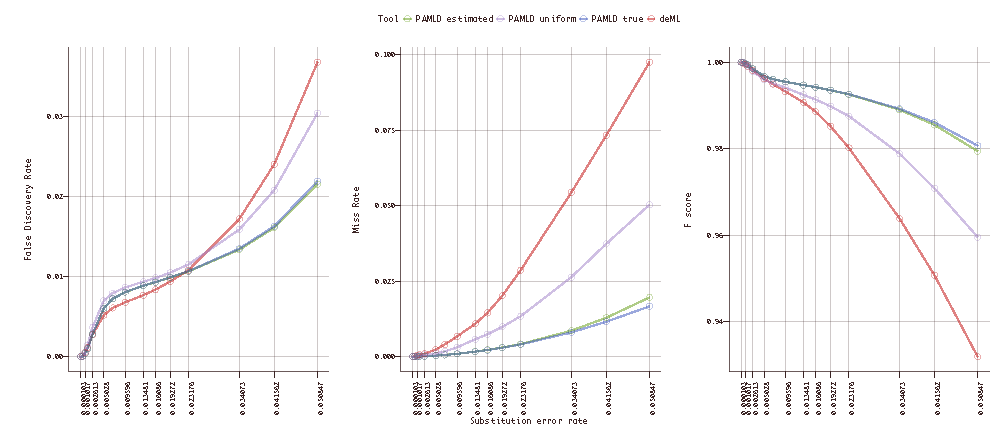
\includegraphics[keepaspectratio,scale=1]{../plot/9_unclassified_accuracy_0550}
\caption{\footnotesize{\textbf{Accuracy for unclassified reads.} } }
\label{fig:09}
\end{figure*}

\begin{figure*}[htbp]
\centering
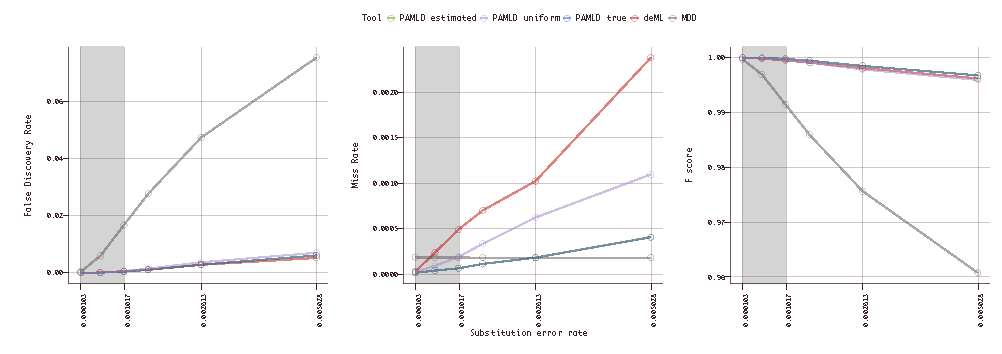
\includegraphics[keepaspectratio,scale=1]{../plot/10_unclassified_accuracy_0060_mdd}
\caption{\footnotesize{\textbf{Accuracy for unclassified reads closeup with mdd.} } }
\label{fig:10}
\end{figure*}

\begin{figure*}[htbp]
\centering
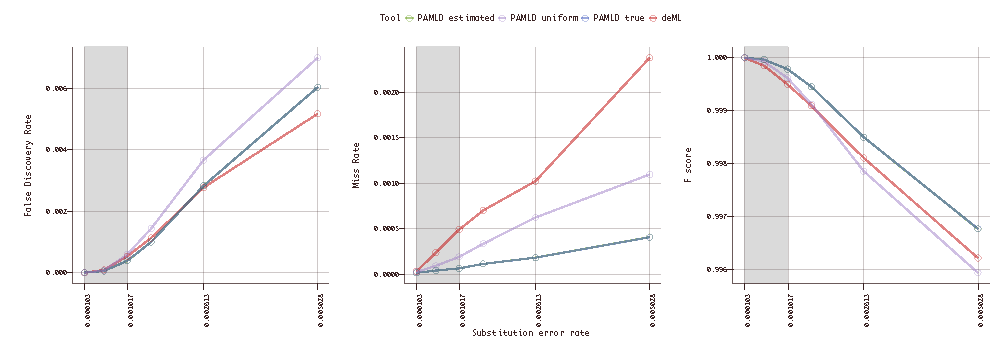
\includegraphics[keepaspectratio,scale=1]{../plot/11_unclassified_accuracy_0060}
\caption{\footnotesize{\textbf{Accuracy for unclassified reads closeup.} } }
\label{fig:11}
\end{figure*}

\begin{figure}[htbp]
\centering
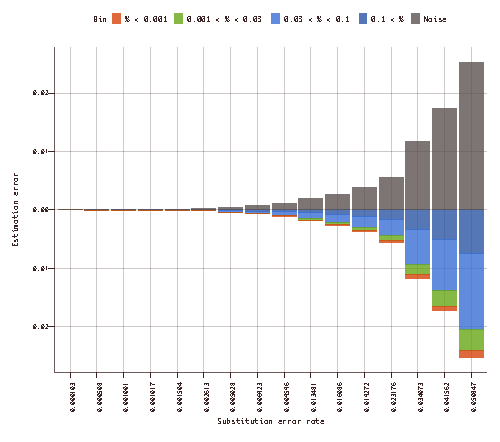
\includegraphics[keepaspectratio,scale=1]{../plot/12_prior_estimation_error_0550_binned}
\caption{\footnotesize{\textbf{Error in prior estimation binned by true barcode prior. } } }
\label{fig:12}
\end{figure}

\begin{figure}[htbp]
\centering
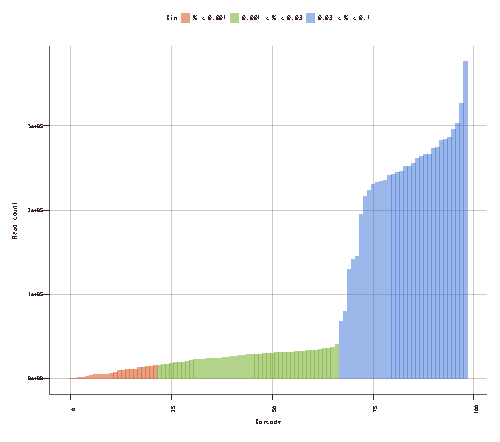
\includegraphics[keepaspectratio,scale=1]{../plot/13_barcode_distribution}
\caption{\footnotesize{\textbf{Barcode true prior distribution. } } }
\label{fig:13}
\end{figure}

\begin{figure*}[htbp]
\centering
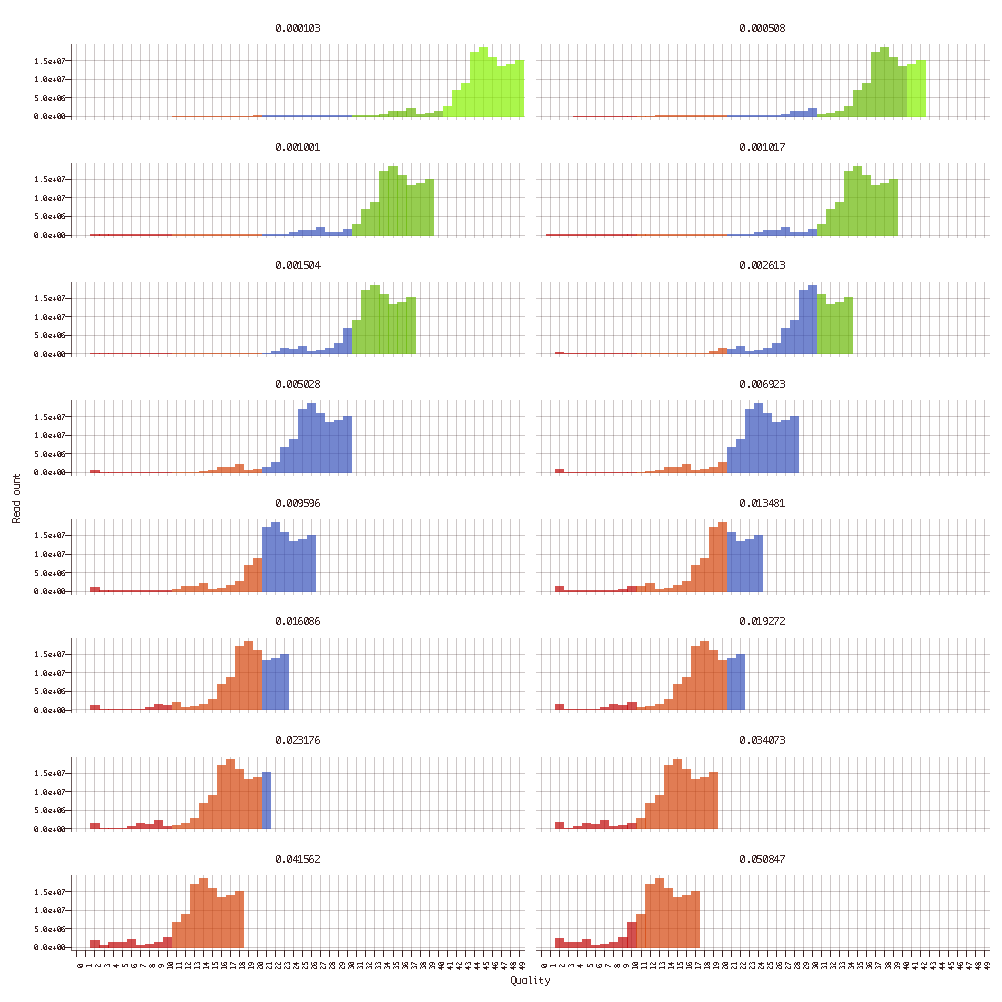
\includegraphics[keepaspectratio,scale=1]{../plot/14_quality_distribution_by_rate_0550}
\caption{\footnotesize{\textbf{Basecall quality distribution for barcode cycles. } } }
\label{fig:14}
\end{figure*}

\begin{figure}[htbp]
\centering
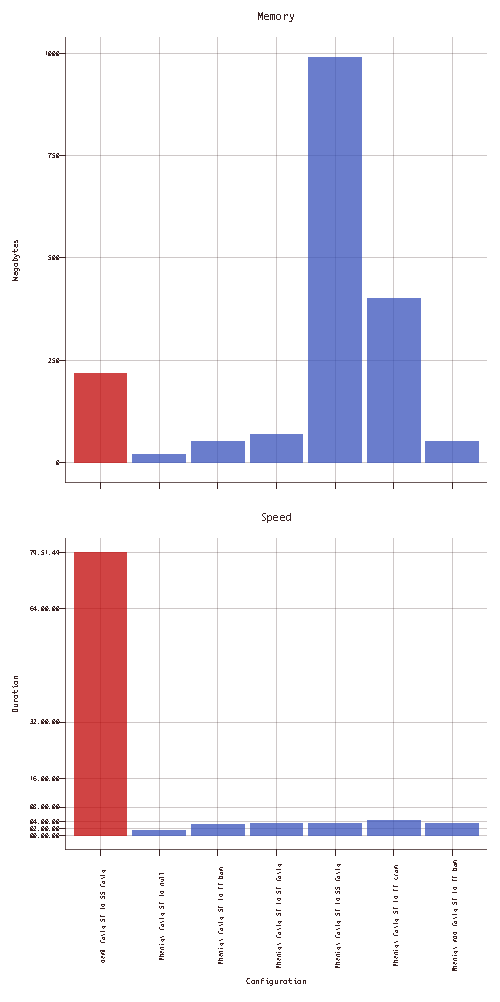
\includegraphics[keepaspectratio,scale=1]{../plot/15_speed_memory}
\caption{\footnotesize{\textbf{Speed and memory benchmarks. } } }
\label{fig:15}
\end{figure}

\begin{figure*}[htbp]
\centering
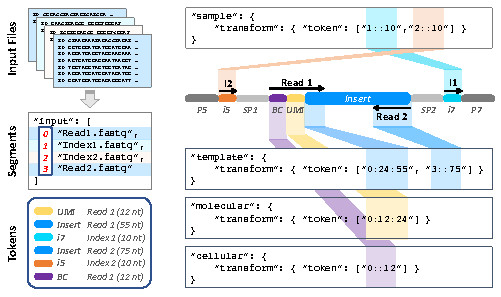
\includegraphics[keepaspectratio,scale=1]{Illumina_tokenization}
\caption{\footnotesize{\textbf{Tokenizing a standard illumina read} Example of tokenization syntax for a paired end input read with a sample barcode composed of two 10 nucleotide long segments and a 12 nucleotide long molecular barcode. } }
\label{fig:16}
\end{figure*}

\begin{figure}[htbp]
\centering
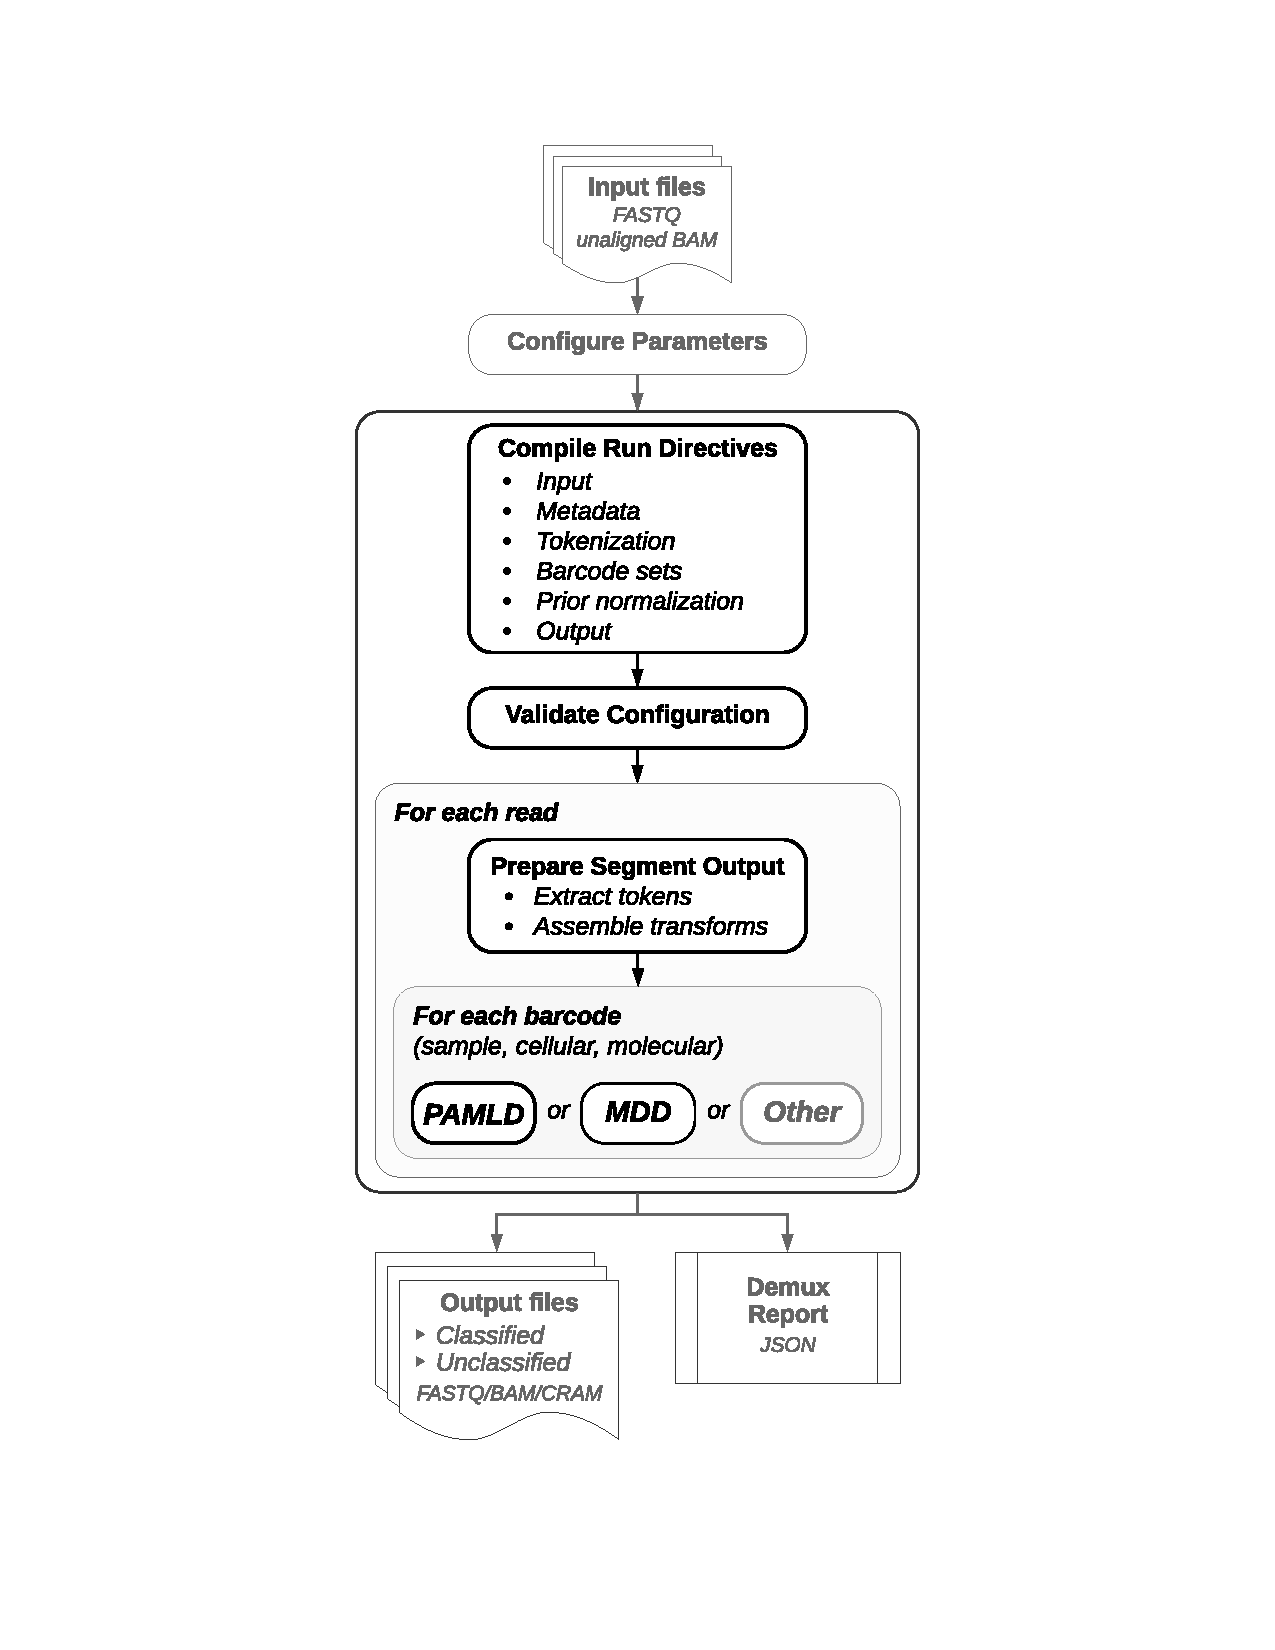
\includegraphics[keepaspectratio,scale=1]{pipeline_overview}
\caption{\footnotesize{\textbf{Pheniqs pipeline architecture} The class hirarchy allows to implement a new decoding algorithm by implementing a few methods in a derived class. } }
\label{fig:17}
\end{figure}

\begin{figure}[htbp]
\centering
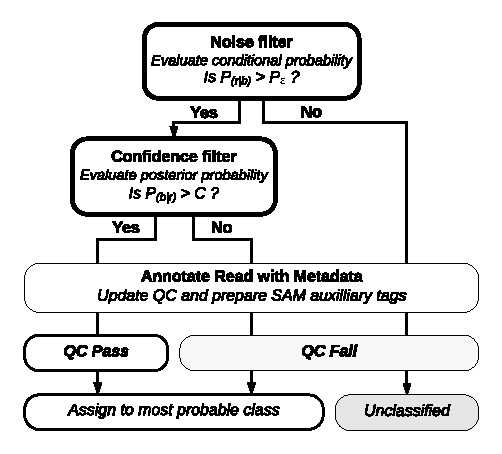
\includegraphics[keepaspectratio,scale=1]{pamld}
\caption{\footnotesize{\textbf{PAMLD decoding} Reads that fail the \emph{noise filter} are classified as noise without further consideration. Reads that fail the \emph{confidence filter} are classified but marked as \emph{qc fail} so the confidence threashold can be reconsidered at a later stage.} }
\label{fig:18}
\end{figure}

\end{document}
